% File: Glossario.tex
% Created: 2014-11-07
% Author: Tesser Paolo
% Email: p.tesser921@gmail.com
% 
%
% Modification History
% Version	Modifier Date	Author			Change
% ====================================================================
% 0.0.1	2014-11-07	Tesser Paolo		creato il file e inclusi i vari input necessari alla compilazione del documento
% ====================================================================
% 0.0.2	2014-11-08	Tesser Paolo		ridefiniti i comandi opportunamente per il glossario
%
%
%

% File: Packages.tex
% Created: 2014-11-07
% Author: Tesser Paolo
% Email: p.tesser921@gmail.com
% 
%
% Modification History
% Version	Modifier Date	Author			Change
% ====================================================================
% 0.0.1	2014-11-08	Tesser Paolo		inseriti package per la gestione ordinario del template
% ====================================================================
% 
%
%
%

\documentclass[11pt,a4paper]{article}

\usepackage{titlesec} % package per le sezioni a quattro indici
\usepackage[left=3.5cm,right=3.5cm,top=3.1cm,bottom=2.6cm]{geometry}
\usepackage[italian]{babel}
\usepackage[utf8]{inputenc}
\usepackage{lastpage}
\usepackage[T1]{fontenc}

\usepackage{geometry}
\geometry{a4paper}

\usepackage{fancyhdr} % package di style per  l/c/rhead l/rfoot
\pagestyle{fancy}

\usepackage{graphicx} % package per la gestione delle immagini
\usepackage{color} % sempre per i colori

\usepackage{hyperref}
\hypersetup{
	colorlinks=true,
	linkcolor=black,
	urlcolor=linkcolor
}

\usepackage{longtable}
\usepackage{tabularx} % package meno complesso per la gestione delle tabelle

\usepackage{pdflscape} % package per mettere il foglio in orizzontale (utile in caso di figure che si estendono in orizzontale)


% File: Commands.tex
% Created: 2014-11-07
% Author: Tesser Paolo
% Email: p.tesser921@gmail.com
% 
%
% Modification History
% Version	Modifier Date	Author			Change
% ====================================================================
% 0.0.1	2014-11-08	Tesser Paolo		inserito nuovo comando per generare il titolo del documento
% ====================================================================
% 
%
%

\newcommand{\documentName}{Nome del Documento}
\newcommand{\documentAuthor}{Nome dell'autore}
\newcommand{\documentListAuthor}{
	\begin{itemize}
		\item Cognome1 Nome1
		\item Cognome2 Nome 2
	\end{itemize}
}

\newcommand{\redactionDate}{\today}
\newcommand{\documentScope}{Scopo generico}
% File: Styles.tex
% Created: 2014-11-07
% Author: Tesser Paolo
% Email: p.tesser921@gmail.com
% 
%
% Modification History
% Version	Modifier Date	Author			Change
% ====================================================================
% 0.0.1	aaaa-mm-gg	Cognome Nome
% ====================================================================
% 
%

\begin{document}

	% Command to redifine
	\renewcommand{\documentName}{Glossario di Ingegneria del Software}
	\renewcommand{\documentAuthor}{Tesser Paolo}
	\renewcommand{\redactionDate}{2014-11-07}
	\renewcommand{\documentScope}{Lo scopo del documento è quello di fornire una distribuzione per i termini più utilizzati e significativi nel mondo dell'ingegneria del software.}
	
	% First Page
	% File: FirstPage.tex
% Created: 2014-11-07
% Author: Tesser Paolo
% Email: p.tesser921@gmail.com
% 
%
% Modification History
% Version	Modifier Date	Author			Change
% ====================================================================
% 0.0.1	2014-11-09	Tesser Paolo		inserito intestazione gestita tramite una tabella
% ====================================================================
% 
%


\begin{center}

	\textbf{\Large Informazioni sul documento}
	\vspace{0.5 cm}

	\begin{longtable}{ l | p{6 cm} } % indica la larghezza della colonna di destra
		\textbf{Nome documento} &  {\documentName}\\[0.5 cm]
		\textbf{Data redazione} & {\redactionDate} \\[0.5 cm]
		\textbf{Redattori} & \parbox{\textwidth}{\documentAuthor} \\[0.5 cm]
	\end{longtable}

	\vspace{2 cm}

	\textbf{\Large Sommario} \\
	\documentScope

\end{center}

\pagebreak

	% Index of Pages
	\tableofcontents \pagebreak

	% Content
	% File: Content.tex
% Created: 2014-11-07
% Author: Tesser Paolo
% Email: p.tesser921@gmail.com
% 
%
% Modification History
% Version	Modifier Date	Author			Change
% ====================================================================
% 0.0.1	2014-11-05	Tesser Paolo		inserito input dal file A.tex
% ====================================================================
% 
%

% File: A.tex
% Created: 2014-11-07
% Author: Tesser Paolo
% Email: p.tesser921@gmail.com
% 
%
% Modification History
% Version	Modifier Date	Author			Change
% ====================================================================
% 0.0.1		2014-11-07		Tesser Paolo	inserita sezione
% ====================================================================
% 0.0.2		2015-02-03		Tesser Paolo	sistemata nota Amministratore, Ambiente di lavoro
% ====================================================================
% 0.0.3		2015-03-12		Tesser Paolo	inserito vocabolo: Anamnesi
% ====================================================================
%
\section{A}

\begin{itemize}
	\item \textbf{Ambiente di lavoro}: è ciò che serve ai processi di produzione. \'E composto da:
		\begin{itemize}
			\item persone
			\item ruoli
			\item procedure
			\item infrastrutture
		\end{itemize}
	\noindent
	Esso influisce sulla qualità del processo e del prodotto. Deve essere quindi: completo, ordinato e aggiornato;

	\item \textbf{Amministratore}: è uno dei ruoli di gestione di un progetto. Esso ha il compito di controllare l'ambiente di lavoro e di amministrare le infrastrutture necessarie allo svolgimento del progetto. \newline
	Deve mettere in pratica ciò che le norme chiedono e attraverso sistemi automatizzati le deve fare eseguire senza renderle troppo ingombranti per gli altri membri. Questo lavoro va fatto in maniera preventiva e pro attiva rispetto l'inizio delle attività e del tutto trasparente agli altri componenti. \newline
	A questa figura fanno quindi capo le configurazioni sui sistemi di versionamento e tutta la documentazione che viene redatta. Non attua scelte personali, ma segue quelle concordate con i responsabili;

	\item \textbf{Analisi vs. Progettazione}: [IS] generalmente l'approccio che abbiamo con l'analisi è di tipo top-down in quanto, se non si ha esperienza, non si riescono ad individuare da subito i componenti del sistema. \'E meglio quindi partire dalle richieste del proponente e ricavarne dei casi d'uso e dei requisiti che andranno a raffinarsi sempre di più. \newline
	Per quanto riguarda la progettazione invece si tende ad avere un approccio bottom-up dato che dopo l'analisi si hanno già in mente le componenti principale del sistema. \newline
	Nonostante quanto detto si possono individuare due tipi approccio:
		\begin{itemize}
			\item \textbf{Funzionale}: in questo caso, l'analisi usa prevalentemente il linguaggio naturale, mentre la specifica della progettazione usa linguaggi formali definendo le funzione e il profilo operazionale. Questo implica una progettazione top-down e una programmazione procedurale;
			\item \textbf{Object-oriented}: in questo caso, l'analisi è orientata agli oggetti, ne deriva un uso prevalente di formalismi grafici (Use Case). Questo implica una progettazione bottom-up, basata sul riuso di componenti già esistenti o la realizzazione di componenti riusabili. La programmazione sarà quindi OO.
		\end{itemize}

	\item \textbf{Analisi dinamica}: [VV] la ripetibilità in maniera deterministica è un requisito essenziale per questo tipo di analisi. Si devono utilizzare alcuni tipi di strumenti:
		\begin{itemize}
			\item \textbf{Driver}: componente attiva fittizia che serve a pilotare un parte del programma. (non è ciò che voglio testare)
			\item \textbf{Stub}: componente passiva fittizia per simulare una parte del programma. \'E un sostituto dell cose che devo guardare che restituisce però sempre la risposta giusta;
			\item \textbf{Logger}: componente non intrusivo di registrazione dei dati di esecuzione per analisi dei risultati.
		\end{itemize}
		\noindent
		Ci sono due tipi di approccio che utilizzano questi strumenti: \textbf{top-down} e \textbf{bottom-up}. Vediamo partendo dall'illustrazione seguente.
		\begin{figure}[htbp]
			\centering
			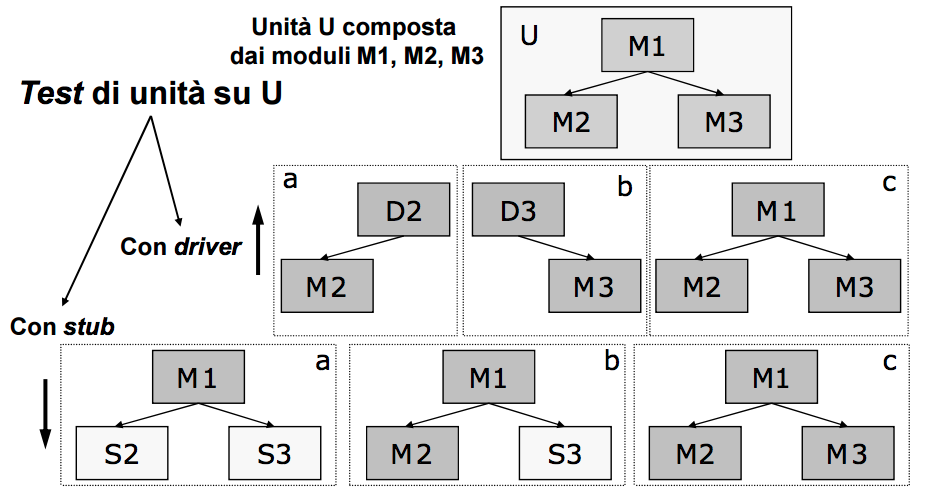
\includegraphics[scale=0.45]{img/stub_driver.png}
			\caption{Architettura Documentazione}
			\label{fig:arch_doc}
		\end{figure}
		Se lavoro in maniera \textbf{top-down} assumo che il comportamento delle foglie sia corretto grazie all'utilizzo di stub. Se invece lavoro in maniera \textbf{bottom-up} rimpiazzo la radice con un driver.




		\item \textbf{Analisi statica}: [VV] attività di verifica applicabile anche sui documenti. Non richiede l'esecuzione di parti del sistema SW. Viene applicata a ogni prodotto di processo e non solo al codice. Si può effettuare con metodi di lettura, impiegati solo per prodotti semplici, e metodi formali, basati sulla prova assistita di proprietà;


	\item \textbf{Analista}: è uno dei ruoli di gestione di un progetto. Esso ha il compito di capire il problema per ottenere i requisiti. Non da la soluzione e spesso non segue fino in fondo la realizzazione del progetto, ma è presente principalmente nella fase iniziale. \newline
	Per cercare i requisiti segue un approccio top-down. Parte infatti ad analizzare quelli espliciti del proponente fino a scinderli in vari sottogruppi gerarchici, trovandone nel frattempo anche di impliciti (il numero maggiore tra le due tipologie);

	\item \textbf{Anamnesi}: nella filosofia platonica è quel processo di reminiscenza che, stimolato dalla percezione degli oggetti sensibili, conduce l'uomo a riscoprire gradualmente nel proprio intelletto (attraverso la conoscenza intellettiva) quelle idee eterne che sono causa e origine del mondo fenomenico. La conoscenza sensibile, distinta dalla conoscenza intellettiva, può dunque offrire a quest'ultima lo spunto per avviare un tale processo;

	\item \textbf{Architettura}: [PR] (definizione) Prima degli anni 80 il termine architettura veniva applicato prevalentemente al sistema fisico. Viene riconosciuto anche nell'ambito software dopo l'evento che riconosceva la disciplina stessa del software engineering. \newline
	Viene definita quindi come una collezione di software e componenti del sistema che dialogano tramite connessioni soggette a vincoli. Questo, quando implementate, andranno a soddisfare le necessità degli stakeholders. Un sistema di architettura software comprende:
		\begin{itemize}
			\item l'insieme di decisioni sull'organizzazione del sistema software;
			\item la selezione degli elementi strutturali e la loro interfaccia con il sistema;
			\item la composizione di queste strutture e il comportamento degli elementi in un sempre più ampio sotto insieme;
			\item lo stile architetturale che guida l'organizzazione. Faccio così perché ottengo questo.
		\end{itemize}
		\noindent
	La decomposizione del sistema in componenti deve essere fatta in maniera top-down. I componenti devono anche essere organizzati in modo da definirne ruoli, responsabilità e interazioni. Buone scelte quindi permettono una buona manutenibilità;

	\item \textbf{Architettura della documentazione}: [DOC] TODO
		\begin{figure}[htbp]
			\centering
			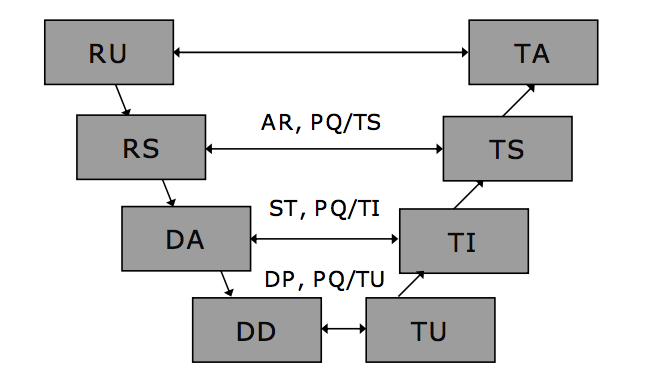
\includegraphics[scale=0.6]{img/v_model_tullio.png}
			\caption{V Model}
			\label{fig:v_model}
		\end{figure}

\end{itemize}
 \pagebreak
% File: B.tex
% Created: 2014-11-07
% Author: Tesser Paolo
% Email: p.tesser921@gmail.com
% 
%
% Modification History
% Version	Modifier Date	Author			Change
% ====================================================================
% 0.0.1		2014-11-07		Tesser Paolo	inserita sezione
% ====================================================================
% 0.0.2		2014-11-10		Tesser Paolo	inserita lista contenente i diversi nomi
% ====================================================================
%

\section{B}

\begin{itemize}
	\item \textbf{Best Practice (migliore prassi)}: modo di fare che per esperienza e per studio si è comportato bene in determinate circostanze, note e specifiche, e abbia mostrato di garantire i risultati migliori;

	\item \textbf{Broken Window Theory}: teoria sociologica, secondo la quale se si impiegano le risorse nella cura e nel rispetto delle cose che già ci sono si ottengono risultati migliori dell'attuazione di norme repressive. Questo perché la gente attua un emulazione del comportamento della comunità;

\end{itemize} \pagebreak
% File: c.tex
% Created: 2014-11-07
% Author: Tesser Paolo
% Email: p.tesser921@gmail.com
% 
%
% Modification History
% Version	Modifier Date	Author			Change
% ====================================================================
% 0.0.1		2014-11-07		Tesser-Paolo	inserita sezione
% ====================================================================
% 
%

\section{C}

\begin{itemize}
	\item \textbf{Casi d'uso}: tecnica usata nei processi di ingegneria del software per effettuare in maniera esaustiva e non ambigua, la raccolta dei requisiti al fine di produrre software di qualità. Consiste nel valutare ogni requisito, focalizzandosi sugli attori che interagiscono col sistema e valutandone le varie interazioni. Il documento dei casi d’uso, individua e descrive gli scenari elementari di utilizzo del sistema, da parte degli attori che si inter facciano con esso.

	\item \textbf{Ciclo di Deming} : è un modello studiato per il miglioramento continuo della qualità in un’ottica a lungo raggio. Serve per promuovere una cultura della qualità che è tesa al miglioramento continuo dei processi e all’utilizzo ottimale delle risorse. Questo strumento parte dall’assunto che per il raggiungimento del massimo della qualità sia necessaria la costante interazione tra ricerca, progettazione, test, produzione e vendita.
Per migliorare la qualità e soddisfare il cliente, le quattro fasi devono ruotare costantemente, tenendo come criterio principale la qualità.
La sequenza logica dei quattro punti ripetuti per un miglioramento continuo è la seguente:
	\begin{itemize}
		\item P: Plan. Pianificazione;
		\item D: Do. Esecuzione del programma, dapprima in contesti circoscritti;
		\item C: Check. Test e controllo, studio e raccolta dei risultati e dei riscontri;
		\item A: Act. Azione per rendere definitivo e/o migliorare il processo.
	\end{itemize}

	\item \textbf{Closure}: nei linguaggi di programmazione è una astrazione che combina una funzione con le variabili libere presenti nell'ambiente in cui è definita. \newline

	\item \textbf{Controllo di versione}:  è la gestione di versioni multiple di un insieme di informazioni. I documenti che vengono gestiti attraverso questa tecnica sono tutti quelli che hanno o necessitano di avere una storia.\newline
Questi strumenti (Git, SVN, Mercurial) ci permettono di muoverci attraverso le varie modifiche che sono state effettuate su file digitali come del codice sorgente, disegni tecnici, documentazione o altro, e, in caso di necessità, ripristinare quelli antecedenti alla versione attuale. \newline
Tutto ciò serve per correggere errori o ritornare a stati in cui non ce ne erano. Ci permette inoltre di procedere su rami diversi in modo da non entrare in conflitto con sezioni stabili dello sviluppo;

\end{itemize} \pagebreak
% File: D.tex
% Created: 2014-11-07
% Author: Tesser Paolo
% Email: p.tesser921@gmail.com
% 
%
% Modification History
% Version	Modifier Date	Author			Change
% ====================================================================
% 0.0.1		2014-11-07		Tesser Paolo	inserita sezione
% ====================================================================
% 0.0.2		2015-02-03		Tesser Paolo	inserita parola Documentazione
% ====================================================================
% 0.0.3		2015-02-10		Tesser Paolo	iniziata stesura vocaboli. Design Pattern
% ====================================================================
%

\section{D}

\begin{itemize}
	\item \textbf{Design Pattern}: [PR] riportano soluzioni a problemi che sono già state sviluppate e che si sono evolute nel corso del tempo in modo tale che il progettista non debba riscoprire ogni volta cose già esistenti. La forma con cui si presentano è succinta e facilmente applicabile. Ci vuole un notevole sforzo ad applicarli, ma ciò viene ripagato dall'incremento nella flessibilità e nella riusabilità della soluzione adottata. \newline
	I pattern non riguardano solo il mondo dei software, ma svariati campi, come ad esempio quelli per la stesura di novelle romantiche o fiabe. \newline
	Per quanto riguarda il mondo software vanno inseriti nella Specifica Tecnica, nella Definizione di Prodotto e nel Piano di Qualifica (?). \newline
	Generalmente un pattern ha quattro elementi essenziali:
		\begin{enumerate}
			\item \textbf{Nome del pattern}: nome simbolico che ci aiuta a inquadrare il problema, permettendoci di ampliare il vocabolario di progetto;
			\item \textbf{Problema}: descrive la situazione al quale applicare il pattern;
			\item \textbf{Soluzione}: descrive gli elementi che costituiscono il progetto, le loro relazioni, responsabilità e collaborazioni;
			\item \textbf{Conseguenze}: sono i risultati e i vincoli che si ottengono applicando il pattern.
		\end{enumerate}
		\noindent
	La classificazione di essi avviene a seconda dello scopo e del loro raggio d'azione.
		\begin{itemize}
			\item \textbf{Scopo}: ciò che il pattern fa. Possono essere di tipo:
				\begin{itemize}
					\item \textbf{Creazionale}: che riguarda il processo di creazione di oggetti;
					\item \textbf{Strutturale}: che riguarda la composizione di classi e oggetti;
					\item \textbf{Comportamentale}: che riguarda il modo in cui le classi o oggetti interagiscono reciprocamente e distribuiscono fra loro le responsabilità;
					\item \textbf{Architetturale}: che riguarda l'architettura globale tra i diversi componenti. Guida la scomposizione in diversi sottoinsiemi. Questi sottoinsiemi sono formati dai design pattern del tipo citato precedentemente.
				\end{itemize}
			\item \textbf{Raggio d'azione}: specifica se il pattern si applica a classi o a oggetti.
		\end{itemize}
		\noindent
	I design pattern ci permettono appunto di risolvere alcuni problemi. Eccone alcuni di essi:
		\begin{itemize}
			\item \textbf{Trovare gli oggetti appropriati}: TO DO;
			\item \textbf{Determinare la granularità degli oggetti}: TO DO;
			\item \textbf{Definire le interfacce degli oggetti}: TO DO;
			\item \textbf{Definire le implementazioni degli oggetti}: TO DO;
			\item \textbf{Mettere in pratica il riuso}: TO DO;
			\item \textbf{Delega}: TO DO;
			\item \textbf{Strutture correlate in compilazione e durante l'esecuzione}: TO DO;
			\item \textbf{Progettare per il cambiamento}: TO DO;
			\item \textbf{Delega}: TO DO;
		\end{itemize}



	\item \textbf{Determinismo}: è la concezione della realtà secondo la quale tutti i fenomeni del mondo sono collegati l’un l’altro e si verificano secondo un ordine necessario e invariabile (il che esclude la presenza del libero arbitrio). \newline
In informatica possiamo applicare questo concetto al fatto che una funzione, o un determinato evento, dia sempre un certo output dato sempre lo stesso input e che quel risultato sarà disponibile in un tempo quantificabile;

	\item \textbf {Diagramma di GANTT}: [PM] è uno degli strumenti di supporto alle attività di pianificazione eseguite dal responsabile di progetto. \newline
Serve per gestire la dislocazione temporale delle attività, per rappresentarne la durata, preventivata e quella poi effettiva, la sequenzialità o il parallelismo. \newline
L'asse delle ascisse è destinata allo scorrere del tempo ed è lunga quanto la durata del progetto. \newline
L'asse delle ordinate invece è riservata alle mansioni che costituiscono il progetto. \newline
Le barre orizzontali rappresentate servono ad indicare la quantità di tempo riservato ad una determinata mansione. Ne deriva quindi un calendario delle attività. \newline
Questo metodo offre quindi un'idea più chiara sull'andamento del progetto e permette di controllare meglio i budget di risorse e conseguentemente i costi;

	\item \textbf {Diagramma di PERT}: (Programme Evaluation and Review Technique) [PM] è uno degli strumenti di supporto alle attività di pianificazione eseguite dal responsabile di progetto. \newline
Serve per arricchire le informazioni date dal diagramma di Gantt. In esso vengono gestite principalmente le dipendenze tra un'attività e un'altra, andando a segnare il tempo di inizio e quello di fine. Tra le attività correlate si potrà dunque verificare se è presente dello \textbf{Slack}, cioè del tempo di margine in caso l'attività precedente non riesca ad essere eseguita nei tempi prefissati. Bisogna stare attenti a come si gestisce ciò perché molto slack causa inattività e non consente ritardo finale.   \newline
Questa tecnica, congiunta allo studio del Cammino critico, permette di visualizzare meglio i collegamenti tra le varie attività e consenti di valutare più facilmente i percorsi critici;

	\item \textbf{Disciplina}: insieme di regole e procedure che attuate conducono a un risultato conforme a determinate aspettative;
	\item \textbf{Disciplinato}: fissato un principio, lo segue sempre senza aggiungere o fare cose che non sono state regolamentate precedentemente da norme di gruppo;
	\item \textbf{Documentazione}: [AM] riguarda tutto ciò che documenta le attività di un progetto, riguardo al prodotto e al processo.
	Per essere utile deve sempre essere disponibile, corretta nei contenuti, verificata, approvata e aggiornata. La diffusione di questi documenti deve essere controllata. Ogni documento infatti deve avere una lista di distribuzione, coerente con i suoi scopi, per non generare offuscamento in chi la riceve.
	\item \textbf{Duck typing}: nei linguaggi di programmazione ad oggetti si riferisce ad uno stile di tipizzazione dinamica dove la semantica di un oggetto è determinata dall'insieme corrente dei suoi metodi e dalla sue proprietà piuttosto che dal fatto di estendere una particolare classe o implementare una specifica interfaccia. \newline
Alcuni linguaggi a cui si riesce ad applicare bene questo principio sono JavaScript o PHP.
Il nome si riferisce al duck test attribuito a James Whitcomb Riley il quale si può esporre attraverso la frase: ``Quando vedo un uccello camminare come un'anatra, nuotare come un'anatra e fare il verso come l'anatra, posso chiamare quell'uccello anatra.".

\end{itemize}
 \pagebreak
% File: F.tex
% Created: 2014-11-07
% Author: Tesser Paolo
% Email: p.tesser921@gmail.com
% 
%
% Modification History
% Version	Modifier Date	Author			Change
% ====================================================================
% 0.0.1		2014-11-07		Tesser Paolo	inserita sezione
% ====================================================================
% 
%

\section{F}

\begin{itemize}
	\item \textbf{Efficacia}: è la capacità di raggiungere l'obiettivo specifico che si cercava di raggiungere applicando una determinata azione. \newline
Viene determinata dal grado di conformità del prodotto rispetto alle norme vigenti e agli obiettivi prefissati;

	\item \textbf{Efficienza}: è la capacità di produrre qualcosa, impiegando il minor numero di risorse che siano esse tempo, denaro o persone durante l'esecuzione delle attività richieste; \newline

\end{itemize} \pagebreak
% File: F.tex
% Created: 2014-11-07
% Author: Tesser Paolo
% Email: p.tesser921@gmail.com
% 
%
% Modification History
% Version	Modifier Date	Author			Change
% ====================================================================
% 0.0.1		2014-11-07		Tesser-Paolo	inserita sezione
% ====================================================================
% 
%

\section{F}
	\begin{itemize}

		\item \textbf{Forme di analisi}: [VV] esistono due principali forme di analisi per effettuare la verifica:
			\begin{itemize}
				\item \textbf{Analisi statica}: non richiede l'esecuzione di alcuna parte del prodotto SW, viene quindi maggiormente impiegata quando il sistema non è ancora disponibile;
				\item \textbf{Analisi dinamica}: richiede l'esecuzione del programma. Viene effettuata tramite prove e test. Questa viene usata sia nelle attività di verifica sia di validazione.
			\end{itemize}

		\item \textbf{Framework}: [PR] insieme integrato di componenti SW prefabbricate. Prima della OO erano chiamate librerie. Sono bottom-up perché fatti da codice già sviluppato, ma anche top-down perché impongono uno stile architetturale. Sono comodi come base di diverse applicazioni entro un dato dominio;

	\end{itemize} \pagebreak
% File: A.tex
% Created: 2014-11-07
% Author: Tesser Paolo
% Email: p.tesser921@gmail.com
% 
%
% Modification History
% Version	Modifier Date	Author			Change
% ====================================================================
% 0.0.1	2014-11-07	Tesser-Paolo		inserita sezione 
% ====================================================================
% 
%

\section{G} \pagebreak
% File: H.tex
% Created: 2014-11-07
% Author: Tesser Paolo
% Email: p.tesser921@gmail.com
%
%
% Modification History
% Version	Modifier Date	Author			Change
% ====================================================================
% 0.0.1		2014-11-07		Tesser-Paolo	inserita sezione
% ====================================================================
%
%

\section{H} % (fold)
\label{sec:h}

% section h (end) \pagebreak
% File: I.tex
% Created: 2014-11-07
% Author: Tesser Paolo
% Email: p.tesser921@gmail.com
%
%
% Modification History
% Version	Modifier Date	Author			Change
% ====================================================================
% 0.0.1		2014-11-07		Tesser-Paolo	inserita sezione
% ====================================================================
% 0.0.2		2015-02-05		Tesser Paolo	inseriti vocaboli: Infrastruttura
% ====================================================================
% 0.0.3		2015-02-11		Tesser Paolo	inseriti vocaboli: Idioma
% ====================================================================
% 0.0.4		2015-03-11		Tesser Paolo	inserito vocabola: Ingegneria dei Requisiti
% ====================================================================
%

\section{I}

\begin{itemize}
	\item \textbf{Idioma}: [PR] è una soluzione specifica ad un linguaggio. Legato quindi alla tecnologia. Esso rinuncia alla genericità della soluzione basata su un design pattern a favore di un implementazione che sfrutta le caratteristiche e le potenzialità del linguaggio;

	\item \textbf{Incremento}: procedere in questo modo significa aggiungere ad un impianto base. Si inserisce, ma non si toglie;


	\item \textbf{Infrastruttura}: [AM] è l'insieme dei servizi offerti sotto la responsabilità dell'amministratore, necessaria allo svolgimento di un progetto. Questa molte volte è trasversale, in parte o totalmente, a più progetti. \'E composta dalle risorse HW (server, rete, postazione di lavoro) e da quelle SW (ambiente di sviluppo, prova, gestione, documentazione);


	\item \textbf{Ingegneria dei requisiti}: [IR] è uno dei primi temi che riguarda i processi di sviluppo (primari). Di solito richiede un ampio insieme di conoscenza. Secondo ISO 12207 non è un processo a se stante, ma un insieme di attività chiave del processo di sviluppo. I requisiti SW sono uno, ma non il solo, dei principali prodotti di tale attività. Le attività necessarie sono quelle di:
		\begin{itemize}
			\item \textbf{Analisi}: consiste nell'analisi dei bisogni e delle fonti, nella classificazione dei requisiti, nella modellazione concettuale del sistema (Use Case), nell'assegnazione dei requisiti a parti distinte del sistema e nella negoziazione con il committente e con i sotto-fornitori;
			\item \textbf{Specifica di verifica e validazione}: consiste nella predisposizione di revisioni interne/esterne e nella predisposizione di prove e dimostrazioni.
		\end{itemize}
	\noindent
	Oltre a queste attività presenti nel processo di sviluppo, vengono coinvolti altri processi:
		\begin{itemize}
			\item \textbf{Documentazione}: processo attraverso il quale si va a redigere lo studio di fattibilità e l'analisi dei requisiti;
			\item \textbf{Gestione e manutenzione dei prodotti}: processo che coinvolge le attività di tracciamento dei requisiti, di impostazione e gestione della configurazione e di gestione dei cambiamenti, cioè l'insieme di attività che consentono di passare da uno stato p a uno stato q, creando consapevolezza e responsabilità;
		\end{itemize}

	\item \textbf{Inspection}: [VV][analisi statica] TODO

	\item \textbf{Iterazione}: procedere in questo modo significa operare raffinamenti o rivisitazioni. A differenza della tecnica incrementale, questa può essere distruttiva. \newline
Devo inoltre fissare un numero preciso di iterazioni da compiere e per farlo ha bisogno di condizioni di uscita forti dal ciclo;

\end{itemize} \pagebreak
% File: L.tex
% Created: 2014-11-07
% Author: Tesser Paolo
% Email: p.tesser921@gmail.com
%
%
% Modification History
% Version	Modifier Date	Author			Change
% ====================================================================
% 0.0.1		2014-11-07		Tesser-Paolo	inserita sezione
% ====================================================================
%
%

\section{L}

\begin{itemize}
	\item \textbf{Lambda Calcolo}: TO DO;

\end{itemize} \pagebreak
% File: K.tex
% Created: 2014-11-07
% Author: Tesser Paolo
% Email: p.tesser921@gmail.com
%
%
% Modification History
% Version	Modifier Date	Author			Change
% ====================================================================
% 0.0.1		2014-11-07		Tesser-Paolo	inserita sezione
% ====================================================================
%
%

\section{K} % (fold)
\label{sec:k}

% section k (end) \pagebreak
% File: M.tex
% Created: 2014-11-07
% Author: Tesser Paolo
% Email: p.tesser921@gmail.com
% 
%
% Modification History
% Version	Modifier Date	Author			Change
% ====================================================================
% 0.0.1	2014-11-07	Tesser-Paolo		inserita sezione 
% ====================================================================
% 0.0.2	2014-11-10	Tesser Paolo		inserita lista con aggiunta di alcune voci
%
%
%

\section{M}

\begin{itemize}
	\item \textbf{MEAN} : si riferisce alle iniziali delle quattro componenti (free e open source) per la costruzione di siti web dinamici. \\
In particolare è uno stack JavaScript per creare applicazioni web. \\
I componenti sono:
	\begin{itemize}
		\item Mondo DB : a NoSQL database;
		\item Express.js : un framework per applicazioni web costrutito in Node.js;
		\item Angular.js : un framework basato sul design pattern MVC per web app;
		\item Node.js : una piattaforma software per gestire servizi web scalabili.
	\end{itemize}

	\item \textbf{Metrica di progetto (Metrics)} : sistema di misurazione composto da valori e metodi per valutarli in maniera oggettiva; 
	
	\item \textbf{Milestone} : 

	\item \textbf{Modelli agili} : è uno dei modelli di ciclo di vita del SW. \\
Nell'idea pura della metodologia agile viene perso il legame con l'ingegneria del software.
Quello che viene proposto infatti è che le persone sono più importanti dei processi e degli strumenti imposti. Di seguito sono riportati i quattro principi fondanti:
		\begin{enumerate}
			\item gli individui e le interazioni tra di essi sono più importanti dei processi e degli strumenti;
			\item un sofware funzionante piuttosoto che una documentazione comprensiva;
			\item collaborazione con il cliente piuttosto che una negoziazione contrattuale;
			\item adattarsi ai cambiamenti piuttosto che seguire un piano preciso e rigido.
		\end{enumerate}
Questo modello ha come obiettivi quelli di riuscire a dimostrare costantemente al cliente quanto è stato fatto. Ciò da maggiore soddisfazione agli sviluppatori che vedono in breve tempo l'avanzamento del risultato finale. \\
Alcune tecniche agili sono: Scrum (caos organizzato) e Kanban (just-in-time).

	\item \textbf{Modello a componenti} : è uno dei modelli di ciclo di vita del SW. Nasce dall'osservazione che molto di quello che ci serve esiste già e molto di quello che faremo ci servirà ancora. \\
Generalmente costa meno come approccio e, se è stato fatto bene il componente che andremo ad integrare, ci sarà una buona probabilità che sia già testato.

	\item \textbf{Modello evolutivo} : è uno dei modelli di ciclo di vita del SW. Esso aiuta a rispondere a bisogni non inizialmente preventivabili. Non si sa dove si vuole andare, ma si procede migliorando. \\
Può richiedere il rilascio e il mantenimento di più versioni esterne in parallelo che consentono una presenza molto vasta sul mercato ,ma ciò può essere estremamente costoso se il prodotto è di tipo commerciale. Alcuni esempi di ciò riguardano Google Chrome e Firefox.

	\item \textbf{Modello incrementale} : è uno dei modelli di ciclo di vita del SW. Prevede rilasci multipli e successivi nei quali avviene un incremento di funzionalità. \\
Alcune fasi però, come l'analisi e la progettazione, non vengono ripetute. Solo la realizzazione assume carattere incrementale iniziando dai requisiti essenziali per poi terminare con quelli desiderabile. In tal modo, già dopo non troppo tempo, si possono mostrare i risultati al commitente e ricevere dei feedback. \\
Così è più facile e meno costoso effettuare dei miglioramenti o dei raffinamenti se necessario;

	\item \textbf{Modello sequenziale (a cascata)} : è uno dei modelli di ciclo di vita del SW più consolidati e autoritari. Prevede una successione di fasi rigidamente sequenziali, non ammettendo ritorni a stati precedenti. Se si verificano eventi eccezionali, essi faranno ripartire dall'inizio. \\
Per passare da uno stato ad un altro vengono introdotte delle PRE e delle POST condizioni molto forti definite all'origine. Le fasi previste sono: Analisi, Progettazione, Realizzazione, Manutenzione. Esse sono distinte e non si sovrappongono. \\
Questo modello però pecca di eccessiva rigidità e spesso il commitente non sa da subito quali sono le sue esigenze in maniera precisa.\\
Ci sono quindi delle correzioni che si possono apportare per renderlo più flessibile. Si può fare della prototipazione solo per capire meglio i requisiti o attuare dei ritorni, in modo che ogni ciclo di ritorno raggruppo delle sottosequenze di fasi;

	\item \textbf{Modello a spirale} : è uno dei modelli di ciclo di vita del SW. Viene impiegato in progetti fortemente innovativi perchè si ha un miglior controllo dei rischi (risk driven). \\
Si attua mediante cicli interni rapidi e ripetuti che consistono in analisi e sviluppo di prototipi, mentre per i cicli esterni si può aderire a un qualsiasi degli altri modelli. \\
Richiede quindi forte interazione tra il commitente e il fornitore. Le fasi presenti sono: definizione degli obiettivi, l'analisi dei rischi, sviluppo e validazione, pianificazione per poi riprendere dall'inizio;

\end{itemize} \pagebreak
% File: N.tex
% Created: 2014-11-07
% Author: Tesser Paolo
% Email: p.tesser921@gmail.com
%
%
% Modification History
% Version	Modifier Date	Author			Change
% ====================================================================
% 0.0.1		2014-11-07		Tesser-Paolo	inserita sezione
% ====================================================================
% 0.0.2		2015-02-05		Tesser Paolo	inseriti vocaboli: Norme di progetto
% ====================================================================
%

\section{N} % (fold)
\label{sec:n}
	\begin{itemize}
		\item \textbf{Norme di progetto}: sono le linee guida per le attività di sviluppo e devono essere in larga misura automatizzate. Una norma può essere:
			\begin{itemize}
				\item \textbf{regola}: ed in tal caso la sua applicazione è obbligatoria, richiedendone il rispetto prima e accertato dopo. Di solito sono convenzioni di cui si riconosce la necessità e convenienza;
				\item \textbf{raccomandazione}: una prassi desiderabile, senza però ne venga verificato il rispetto.
			\end{itemize}
			\noindent \newline
		Di esse ne deve essere identificato il contesto, in quanto non tutto può essere regolamentato. Inoltre troppo regole sono di difficile attuazione e verifica. \newline
		Le norme possono riguardare diversi ambiti. Alcuni di essi vengono descritti di seguito:
			\begin{itemize}
				\item \textbf{norme di codifica}: una buona leggibilità del codice ne permette una più facile verifica, manutenzione e portabilità. Bisogna accertarsi in particolare che ciò che viene codificato sia comprensibile a distanza di tempo e a chi non lo ha prodotto;
				\item \textbf{convenzioni sui nomi}: per far si che ci sia omogeneità tra le diverse componenti che vengono sviluppate, ci deve essere un attenzione rigorosa su come identifichiamo ciò che è presente nel nostro repository e all'interno dei file stessi;
				\item \textbf{indentazione del codice}: in modo da poter evidenziare facilmente la struttura e i costrutti di programmazione. Non bisogna sottovalutare la lunghezza delle linee e l'ampiezza dell'indentazione;
				\item \textbf{intestazione del codice}: serve a identificare e collocare ciascuna unità nel modo corretto. Inoltre serve per tenere traccia delle modifiche e del perché sono state fatte. Di solito va inserita nell'header del file e deve contenere: dati relativi all'unità, responsabilità, Copyright, copyleft, avvertenze e un registro delle modifiche.
			\end{itemize}
			\noindent
		Questo insieme di regole servono perché il codice illeggibile è irritante, modificarlo costa tempo e denaro (e spesso rischioso). Deve quindi fungere da risorsa e non da ostacolo. \newline
		Per fare questo inoltre c'è bisogno di una forte disciplina di programmazione attua a produrre codice che non generi errori fatali o warning. Ciò si può attuare più facilmente apportando alcune restrizioni sul linguaggio utilizzato, usando i costrutti più facilmente testabili, robusti e leggibili anche a scapito di maggiore potenza e velocità;


	\end{itemize}
% section n (end) \pagebreak
% File: O.tex
% Created: 2014-11-07
% Author: Tesser Paolo
% Email: p.tesser921@gmail.com
% 
%
% Modification History
% Version	Modifier Date	Author			Change
% ====================================================================
% 0.0.1	2014-11-07	Tesser-Paolo		inserita sezione 
% ====================================================================
% 
%

\section{O} \pagebreak
% File: P.tex
% Created: 2014-11-07
% Author: Tesser Paolo
% Email: p.tesser921@gmail.com
%
%
% Modification History
% Version	Modifier Date	Author			Change
% ====================================================================
% 0.0.1		2014-11-07		Tesser-Paolo	inserita sezione e lista contenente le voci del glossario
% ====================================================================
%
%

\section{P}

\begin{itemize}
	\item \textbf{Piano di Progetto}: [PM] è uno dei documenti esterni da redarre. Viene steso dal responsabile di progetto. \newline
In esso vengono fissate le risorse disponibili, la suddivisione delle attività e il loro calendario. \newline
Si deve cercare di organizzare le attività in modo da produrre risultati utili per valutare con efficacia il grado di avanzamento del lavoro. \newline
Serve inoltre fissare delle milestone come punti critici o finali delle attività. \newline
La struttura tipica di questo documento segue questo schema:
	\begin{enumerate}
		\item Introduzione (scopo e struttura);
		\item Organizzazione del progetto;
		\item Analisi dei rischi, maggiori sono i rischi maggiori saranno i punti di controllo. \newline
Le tipologie di rischi possibili sono: a livello tecnologico, a livello del personale, a livello organizzativo, a livello dei requisiti (quello che causa più probabilità di fallimento) e a livello di valutazione dei costi;
		\item Risorse necessarie e risorse disponibili (HW e SW);
		\item Suddivisione del lavoro (Work Breakdown);
		\item Calendario delle attività;
		\item Meccanismi di controllo e di rendicontazione.
	\end{enumerate}
 

	\item \textbf{Pro attivi}: al contrario di re-attivi, si è pro attivi quando si cerca di risolvere un problema prima che esso si manifesti. In particolare riguarda gli errori che si potranno commettere e cercare di prevenirli. \newline
Agire prima permette di ridurre i costi oltre al fatto di capire meglio ciò che si sta facendo e garantire una migliore qualità del prodotto;

	\item \textbf{Procedura}: in generale è l'insieme di regole e norme da svolgere in maniera sequenziale per ottenere un determinato risultato. \newline
In informatica (funzione) è un blocco di istruzioni che a partire da un certo input restituiscono un determinato output;

	\item \textbf{Processo}:  in generale è una rete di cambiamenti, attività o azioni collegate tra loro per la creazione, la verifica, la manutenzione, ecc di un prodotto. \newline
Durante il ciclo di vita del software tramite un processo si attua la transizione tra uno stato e l'altro. Nel particolare vengono chiamati processi di ciclo di vita. \newline
In Informatica si intende un'istanza di un programma in esecuzione in modo sequenziale. \newline
A differenza di un programma, esso è un'entità dinamica, che dipende dai dati che vengono elaborati, e dalle operazioni eseguite su di essi. Il processo è quindi caratterizzato, oltre che dal codice eseguibile, dall'insieme di tutte le informazioni che ne definiscono lo stato, come il contenuto della memoria indirizzata, i thread, i descrittori dei file e delle periferiche in uso;
	
	\item \textbf{Progettista}: è uno dei ruoli di gestione di un progetto. \newline
Esso ha il compito di trovare la migliore soluzione per i requisiti trovati dall'analista. Per fare ciò generalmente utilizza un approccio bottom-up. \newline
Non si occupa dell'implementazione, compito spettante invece al programmatore. La sua presenza nel progetto dura in genere fino alla manutenzione.
	
	\item \textbf{Programmatore}: è uno dei ruoli di gestione di un progetto. 	\newline
Esso ha il compito di implementare le soluzioni trovate dal progettista. Non si deve inventare nulla proprio perché quello che deve fare è già stato fissato in precedenza. Partecipano sia allo sviluppo che alla manutenzione.

	\item \textbf{Programma}: è un insieme di istruzioni che, una volta eseguite su un computer, produce soluzioni per una data classe di problemi automatizzati;

\end{itemize} \pagebreak
% File: Q.tex
% Created: 2014-11-07
% Author: Tesser Paolo
% Email: p.tesser921@gmail.com
%
%
% Modification History
% Version	Modifier Date	Author			Change
% ====================================================================
% 0.0.1		2014-11-07		Tesser-Paolo	inserita sezione
% ====================================================================
% 0.0.2		2015-02-10		Tesser Paolo	inseriti vocaboli: Qualità
% ====================================================================
%

\section{Q}

\begin{itemize}
	\item \textbf{Qualità}: [QS] è l'insieme delle caratteristiche di un'entità (prodotto, processo, servizio) che ne determinano la capacità di soddisfare esigenze espresse e implicite. La qualità serve per intervenire su alcune aree per e la sua visione deve essere:
		\begin{itemize}
			\item \textbf{intrinseca}: conforme con i requisiti e idoneità all'uso (sempre presenti a prescindere);
			\item \textbf{relativa}: deve soddisfare il cliente;
			\item \textbf{quantitativa}: ricevere un livello di qualità per confronto.
		\end{itemize}
		\noindent
		Questi concetti si legano fortemente a quello di valutazione. Servono dunque mezzi oggettivi per dare un valore a ciò che si è fatto. \newline
		La ricetta per raggiungere la qualità (a livello di PDCA) consiste nel pianificare bene ciò che deve essere realizzato e come andrà controllato rispetto agli obiettivi di miglioramento. In seguito bisognerà controllare, per poter conoscere e intervenire in tempo. \newline
		A volte al fornitore è richiesto che il prodotto rispetti alcune norme, sia a livello di prodotti sia di processi in modo che il cliente sia tutelato rispetto all'uso o al valore dei prodotti. \newline
		La qualità dovrà essere quindi: esterna, interna ed in uso. Le prime due sono fortemente connesse e riguardano: le funzionalità, l'affidabilità, l'efficienza, l'usabilità, la manutenibilità e la portabilità. Quella interna sarà fonte di requisiti, anche se non espliciti, e la più vasta rispetto alla interna. Deriva infatti da scelte di progettazione codifica, verifica e che si vede solo attraverso una revisione critica. Quella interna si osserva invece tramite esecuzione del prodotto;

		\item \textbf{Qualità architetturali}: [PR][TO DO];

	\item \textbf{Quantificabile}: di cui è possibile misurarne l'efficacia e l'efficienza, anche a priori;

\end{itemize} \pagebreak
% File: R.tex
% Created: 2014-11-07
% Author: Tesser Paolo
% Email: p.tesser921@gmail.com
%
%
% Modification History
% Version	Modifier Date	Author			Change
% ====================================================================
% 0.0.1		2014-11-07		Tesser-Paolo	inserita sezione
% ====================================================================
% 0.0.2		2015-03-12		Tesser Paolo	inserita voce Requisito
% ====================================================================
%

\section{R}

\begin{itemize}
	\item \textbf{Requisito}: [IR] possono essere espliciti o impliciti. Secondo IEEE, è la condizione necessaria a un utente per risolvere un problema o raggiungere un obiettivo (visione dal lato del bisogno). \'E inoltre la condizione che deve essere soddisfatta o posseduta da un sistema per adempiere a un obbligo (visione dal lato della soluzione). \newline
	Il requisito è dunque necessario per: capire la domanda e capire la risposta;

	\item \textbf{Responsabile}: è uno dei ruoli di gestione di progetto. Esso rappresenta il progetto di tutto il team presso il fornitore e il committente. Viene quindi accentrata la responsabilità di scelta e approvazione. \newline
	Partecipa interamente al ciclo di vita del prodotto e sa sempre (senza bisogno di domandare nulla agli altri membri) a che punto è l'avanzamento delle attività per il raggiungimento degli obiettivi fissati. \newline
	Ha quindi responsabilità sulla pianificazione, sulla gestione delle risorse umane tramite coordinamento e relazioni esterne con il committente. \newline
 	pianificazione consiste nella definizione delle attività che il team dovrà svolgere e l'assegnamento dei tempi di esecuzione per quelle attività riuscendo a determinarne i costi di attuazione, da fornire poi come preventivo al proponente e come consuntivo nella fase finale. \newline
	Ci sono diversi strumenti per lo svolgimento di questo ruolo, come l'utilizzo di Diagrammi di Gantt e di PERT .

	\item \textbf{Ruolo}: è una funzione aziendale assegnata a progetto. E' un servizio che viene svolto per la comunità. Ne esistono di diversi e non tutti ammettono parallelismo. \newline
	Ci sono diversi ruoli che si possono raggruppare più macroscopicamente in quattro gruppi:
	\begin{enumerate}
		\item Sviluppo: ha la responsabilità tecnica e realizzativa;
		\item Direzione: ha la responsabilità decisionale (molto importante);
		\item Amministrazione: ha la responsabilità della gestione dei processi;
		\item Qualità: ha la responsabilità di gestione della qualità.
	\end{enumerate}

\end{itemize}
 \pagebreak
% File: S.tex
% Created: 2014-11-07
% Author: Tesser Paolo
% Email: p.tesser921@gmail.com
% 
%
% Modification History
% Version	Modifier Date	Author			Change
% ====================================================================
% 0.0.1	2014-11-07	Tesser-Paolo		inserita sezione 
% ====================================================================
% 
%

\section{S}

\begin{itemize}
	\item \textbf{Scrum} : 

	\item \textbf{SEMAT} : Software Engineering Method and Theory è una comunità industriale con lo scopo di migliorare le pratiche dell'ingegneria del software, ridefinendola come una discipliana rigorosa;

	\item \textbf{Sistematico} : costante, che fa sempre la stessa cosa in determinate situazioni, applicando un comportamento, che deve tendere ad esser best, ripetitivo;

	\item \textbf{Stakeholder (portatore di interesse)} : è l'insieme di persone coinvolte nel ciclo di vita del SW con influenza sul prodotto. \\
Possono essere chi usa lo usa, chi lo paga o chi lo sviluppa;

\end{itemize} \pagebreak
% File: T.tex
% Created: 2014-11-07
% Author: Tesser Paolo
% Email: p.tesser921@gmail.com
%
%
% Modification History
% Version	Modifier Date	Author			Change
% ====================================================================
% 0.0.1		2014-11-07		Tesser-Paolo	inserita sezione
% ====================================================================
% 0.0.2		2015-03-18		Tesser Paolo	inserito vocabolo: Tecniche di analisi
% ====================================================================
%

\section{T} % (fold)
\label{sec:t}
	\begin{itemize}
		\item \textbf{Tecniche di analisi}: [IS] ci sono diversi approcci per analizzare i bisogni e le fonti di un progetto. Attraverso lo studio del dominio, andando quindi ad osservare i comportamenti dell'utente finale e dell'ambiente d'uso immergendosi nei panni degli utilizzatori. Interagendo con il cliente in maniera il meno invasiva possibile e facendolo in modo strutturato e rendicontabile. Un'altra tecnica è quella di avere dei brain-storming, ma per farlo bisogna che:
			\begin{itemize}
				\item ci sia un gruppo di persone che sono consapevoli di ciò che stanno facendo;
				\item serve un'altra persona che fa da controllore, fissa l'agenda, il tempo e la scaletta;
				\item serve una persona che tenga le minute, cioè i punti salienti.
			\end{itemize}
		\noindent
		Infine può essere fatta anche della prototipazione, che può essere interna (per capire meglio le cose) o esterna (per chiedere al cliente se ciò che sta domandando);

		\item \textbf{Teorema di Dijkstra (1969)}: [VV][analisi dinamica] il test di un programma può rilevare la presenza di malfunzionamenti, ma non dimostrarne l'assenza;

		\item \textbf{Teorema di Howden (1975)}: [VV][analisi dinamica] non esiste un algoritmo che, dato un programma P qualsiasi, generi per esso un test finito ideale;

		\item \textbf{Test}: [VV][analisi dinamica]
			\begin{figure}[htbp]
				\centering
				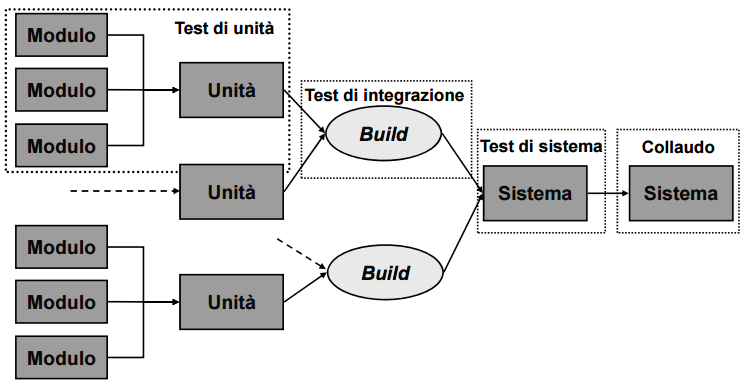
\includegraphics[scale=0.5]{img/composizione_test.png}
				\caption{Composizione Test}
				\label{fig:comp_test}
			\end{figure}

			\begin{itemize}
				\item \textbf{test di unità}: attività di analisi dinamica che si può svolgere con il massimo grado di parallelismo in quanto coinvolge la più piccola parte non ulteriormente scomponibile di un programma. La responsabilità è dello stesso programmatore per le unità più semplici, altrimenti di un verificatore autonomo. Nel primo caso infatti potrebbe esserci conflitto di interesse, meglio quindi peer-programming. Sono i test più costosi. Unità e moduli vengono determinati durante la progettazione di dettaglio e conseguentemente anche il piano di test. La TU è completa quando ha verificato tutte le unità. Piuttosto di tagliare i test di unità, è meglio che il Responsabile di Progetto, tagli i requisiti opzionali. Possono essere di due tipi:
					\begin{itemize}
						\item \textbf{test funzionale (black-box)}: guarda solo l'uscita. Da solo non può accertare correttezza e completezza della logica interna dell'unità. Va quindi necessariamente integrato con test strutturali. Fa riferimento alla specifica dell'unità e utilizza dati di ingresso capaci di provocare l'esito atteso. Si usano delle le classi di equivalenza per non avere infiniti valori di ingresso;
						\item \textbf{test strutturale (white-box)}: verifica la logica interna del codice dell'unità cercando massima copertura. Ciascuna prova deve essere progettata per attivare ogni cammino di esecuzione all'interno del modulo. Ciascuno insieme di dati di ingresso che attivano un percorso costituiscono un caso di prova.
					\end{itemize}

				\item \textbf{test di integrazione}: servono per verificare la costruzione incrementale del sistema. Può essere in parallelo per i componenti che non collaborano tra di loro. In condizioni ottimali, l'integrazione dovrebbe essere prova di problemi. Viene applicata alla componenti specificate nella progettazione architetturale. La loro integrazione costituisce il sistema completo. I problemi che si rilevano durante questi test manifestano difetti di progettazione o insufficiente qualità nei test di unità. Si inizia a integrare la componente che ha meno dipendenze.

				\item \textbf{test di sistema e collaudo}: i primi sono svolti internamente dal fornitore per accertare la copertura dei requisiti SW, mentre i secondi sono supervisionati dal committente per dimostrare la conformità del prodotto sulla base di casi di prova specificati nel o implicati dal contratto. I primi sono di tipo funzionale (black-box) in quanto non dovrebbero richiedere conoscenza della logica interna del software.

				\item \textbf{test di regressione}: rappresentano l'insieme di test necessari ad accertare che la modifica di una parte P di S non causi errori in P o nelle altre parti di S che dipendono da P. Il rischio che degli errori si verifichino cresce tanto più cresce l'accoppiamento fra le diverse parti e al diminuire dell'accoppiamento.

			\end{itemize}







		\item \textbf{Tracciamento dei requisiti}: [DOC] ha il compito di fissare le relazioni tra i prodotti del processo di sviluppo. Vengono usate delle matrici di tracciabilità. Il tracciamento viene fatto in avanti (forward) che indica la completezza e all'indietro (backward) che indica la necessità. I tracciamenti necessari sono i seguenti:
			\begin{itemize}
				\item requisiti utente (capitolato) <-> requisiti software (AdR)
				\item requisiti software <-> descrizione dei componenti (ST)
				\item test di unità <-> moduli di disegno di dettaglio (DdP)
				\item test di integrazione <-> componenti architetturali
				\item test di sistema <-> requisiti software
				\item test di accettazione <-> requisiti utente
			\end{itemize}

	\end{itemize}
% section t (end) \pagebreak
% File: U.tex
% Created: 2014-11-07
% Author: Tesser Paolo
% Email: p.tesser921@gmail.com
%
%
% Modification History
% Version	Modifier Date	Author			Change
% ====================================================================
% 0.0.1		2014-11-07		Tesser-Paolo	inserita sezione
% ====================================================================
%
%

\section{U}

\begin{itemize}

	\item UML: acronimo di Unified Modeling Language, (linguaggio di modellazione unificato), è un linguaggio di modellazione e specifica basato sul paradigma object-oriented. Consente di costruire modelli object-oriented per rappresentare domini di diverso genere. Nel contesto dell’ingegneria del software, viene usato soprattutto per descrivere il dominio applicativo di un sistema software e/o il comportamento e la struttura del sistema stesso.


\end{itemize} \pagebreak
% File: V.tex
% Created: 2014-11-07
% Author: Tesser Paolo
% Email: p.tesser921@gmail.com
% 
%
% Modification History
% Version	Modifier Date	Author			Change
% ====================================================================
% 0.0.1	2014-11-07	Tesser-Paolo		inserita sezione 
% ====================================================================
% 
%

\section{V}

\begin{itemize}
	\item \textbf{Verificatore} : è uno dei ruoli di gestione di un progetto. \\
Necessità come per la categoria dei programmatori di molte unità. Partecipano all'intero ciclo di vita in quanto servono a mantenere la qualità e aiutare a rimuovere gli errori.


\end{itemize} \pagebreak
% File: W.tex
% Created: 2014-11-07
% Author: Tesser Paolo
% Email: p.tesser921@gmail.com
%
%
% Modification History
% Version	Modifier Date	Author			Change
% ====================================================================
% 0.0.1		2014-11-07		Tesser-Paolo	inserita sezione
% ====================================================================
%
%

\section{W}

\begin{itemize}

	\item \textbf{Walkthrough}: [VV][analisi statica] TODO

	\item \textbf{Work Breakdown Structure}: Breakdown significa esplosione, decomposizione. Questa attività serve per identificare tutti i compiti che dovranno essere svolti dai membri di un progetto. I compiti sono appunto delle attività che si compongono di altre sotto attività. Sono unicamente identificate e possono non essere svolte in ordine sequenziale. \newline
Si parte quindi da un macro obiettivo fino a decomporlo in compiti sempre più piccoli (ma non troppo) tali da poter essere assegnati a una singola persona e che essa possa comprenderli facilmente. \newline
Bisogna quindi stare molto attenti sia a non sottostimare il problema, sia a non sovra-stimarlo.

\end{itemize} \pagebreak
% File: Y.tex
% Created: 2014-11-07
% Author: Tesser Paolo
% Email: p.tesser921@gmail.com
%
%
% Modification History
% Version	Modifier Date	Author			Change
% ====================================================================
% 0.0.1		2014-11-07		Tesser-Paolo	inserita sezione
% ====================================================================
%
%

\section{Y} % (fold)
\label{sec:y}

% section y (end) \pagebreak
% File: Z.tex
% Created: 2014-11-07
% Author: Tesser Paolo
% Email: p.tesser921@gmail.com
% 
%
% Modification History
% Version	Modifier Date	Author			Change
% ====================================================================
% 0.0.1	2014-11-07	Tesser-Paolo		inserita sezione 
% ====================================================================
% 
%

\section{Z} \pagebreak


\end{document}